% !TeX root = _main.tex
% ========================================
% 実演と考察
%   いつどこで「発表」したか（12/20など），どういう形式で行ったか，写真や動画？
%   完成品はどこで聞ける？YouTubeリンクなど
%
%   作ってどうだったか，今後の課題など
% ========================================

%1
\section{作品実演の報告}
本章では，本研究で制作した作品の実演内容と，その際に得られた筆者自身の所感，および参加者の意見を整理する．音のみで情報を伝えるという試みにおいて，本作品を実際の聴取環境に置いた際に，音声設計上のどのような点が問題として顕在化したかを整理することを目的としている．

なお，本実演は評価実験を目的としたものではなく，第三者の知覚の傾向を把握するための試みとして位置づけている．

\begin{figure}[t]
    \centering
    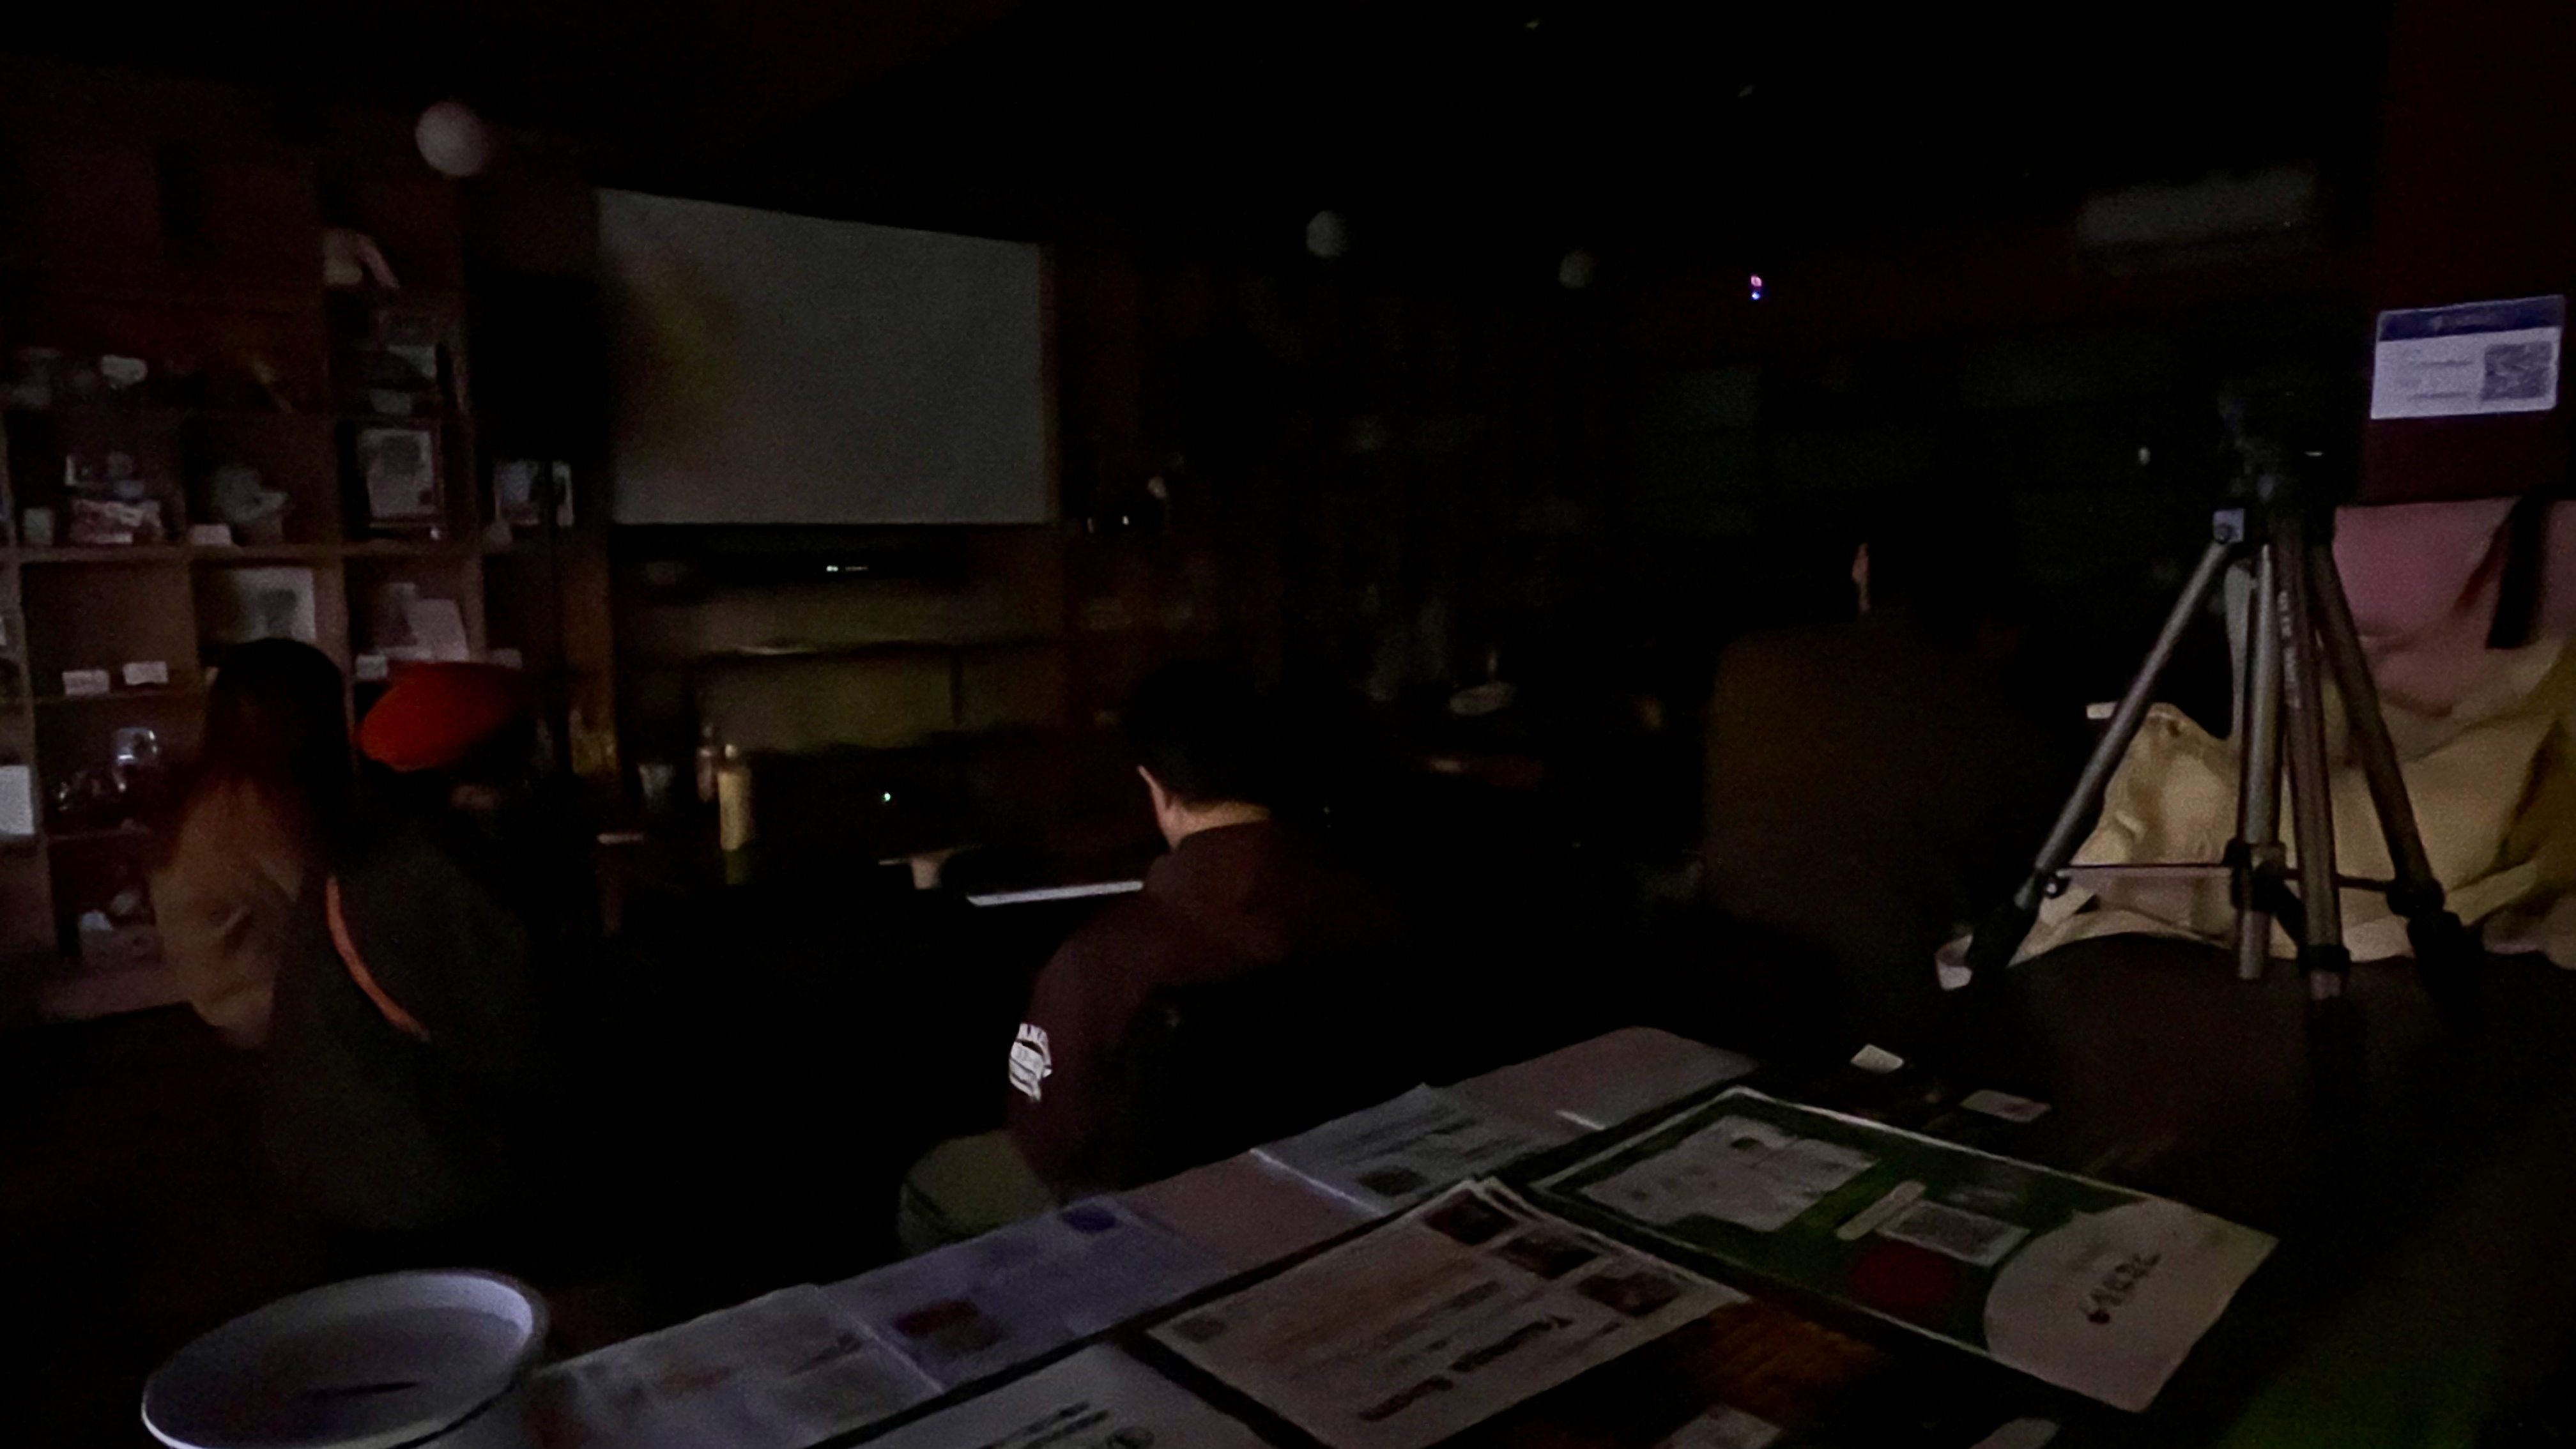
\includegraphics[width=\hsize]{1220oto.png}
    \caption{作品実演の様子}\label{fig:1220oto}
\end{figure}
\subsection{実演の概要と環境}
2025年12月20日に，京都府福知山市の内記新町商店街にある「TsunagaRoom」にて開催された「まちなかで音のとびらを開く会」において，当イベントのプログラムの一環として，参加者を対象に本作品を発表した（\figref{fig:1220oto}）．

本作品は聴覚体験を中心とする構成であるため，視覚情報をできるだけ排した状態での鑑賞を意図し，日が暮れた時間帯である午後5時に，複数人で同時に聴取できるスピーカー出力の形式で，作品発表を計2回行った．また，音だけで情報を伝えるという本研究のテーマにより忠実に従うため，「この物語作品は，音のみで構成されている」という情報のみを示し，事前にあらすじを告知せずに発表を行った．

\subsection{筆者自身の所感}
当イベントでの発表を通じて，作品制作の段階でヘッドホンを用いて聴取していた音と，発表の段階でスピーカーを通じて聴取した音とでは，音量のバランスの感じ方に差異があることを実感した．具体的には，冒頭の雷雨の音声が，作品全体の他の音声と比較して突出して大きく感じられ，全体の音量バランスの問題を確認した．さらに，同一のシーン内において，特定の音声の音量が大きく設定されているために，他の音声が聴こえづらく感じられる箇所も確認された．これにより，目立って大きい音声に気を取られることによって，聴者の世界観の固定が不安定になる可能性が示唆された．

これらの問題はいずれも，作品制作時にヘッドホンで聴取していた際には意識されなかったものであり，制作者の意図する物語的状況の把握が妨げられる可能性があると考えられた．

\subsection{参加者からの意見}
当イベントの参加者からは，「事前にあらすじが知らされていないと，何が起こっているのかの理解がしづらい」という意見が得られた．また，別の参加者からは，知覚の手がかりが音のみに限定されていることにより物語内容の把握が難しいという点に触れつつ，「もっと広い場所など，異なる環境で聴取を行うと，また別の知覚の結果が得られるかもしれない」という旨の意見が示された．

これらの意見を踏まえると，本作品における音声の構成には，製作者の意図を十分に伝えるための設計上の課題が残されていると考えられる．また，聴取環境の違いによって知覚の結果が変化する可能性についての指摘も得られたが，本作品においては，環境条件を変える以前に，音の構成そのものについて再検討の余地がある点が，より大きな課題である．

\subsection{まとめ}
本章では，本作品の実演を通じて得られた参加者の意見と，筆者自身の聴取体験を整理した．その結果，音のみを用いた物語の制作において，現時点の音声の設計では，音を手掛かりとした情報伝達を行うことは容易ではないことが示唆された．

次章では，本章で整理した実演時の結果を踏まえ，音による出来事や感情の表現に関する設計上の課題について考察を行う．

\section{考察と今後の課題}
本作品の制作過程において，効果音がどのような外界の出来事を示すか，また登場キャラクターの鳴き声がどのような感情や態度を示すかについて，エフェクトの付与やボリュームの調整に加え，ピッチやタイミングの制御を通じて表現することを試みた．筆者自身は，これらの音声設計がどのような知覚をもたらし得るかについて，一定の見通しを持って作品制作に取り組んだ．しかし，第三者による作品聴取の機会を踏まえると，制作時と聴取時とでは受け取られ方に差異が生じる可能性があり，制作者の意図した表現が聴取時に十分に共有されない場面が見られた．このことから，制作者がそれぞれの音声がもたらし得る知覚を想定していたとしても，その想定が聴取の場面において同様に成立するとは限らないことが示唆される．

これまでの考察に加え，制作全体を通じて感じられた別の側面について検討すると，聴取時に1つの音声に焦点を当てた場合，それが何らかの物理現象や感情を示しているかを判断することはできても，それが物語の文脈上でどのような意味を持つのかを理解することは，現時点の音声設計では困難であると考えられた．例えば，物語中で風の音が聞こえる場面において，聴取者は風が吹いているという状況自体は理解できるものの，それが別れの切なさや主人公の意思といった物語的意味を担っているかどうかを把握することは容易ではなかったと考えられる．

これらの点を踏まえると，今後の課題として，物語全体の構成を一度に提示する方法だけでなく，より小さな単位で音声表現を検討する必要があると考えられる．本作品は6つの場面で構成される物語となっているが，「食べ物の譲渡」や「登場キャラクター同士の会話」といった，より小さな単位のイベントに焦点を当て，それぞれがどのような内容のイベントとして受け取られ得るかを整理・検討することで，音声設計の改善につなげられる可能性がある．

以上より，本作品を通じて得られた課題として，音のみを用いた物語表現においては，物語全体の完成度を高める以前に，意味的なまとまりを持つ比較的小さな音声イベントが，聴取時にどのように知覚されるかを検討する段階を設ける必要性が示唆された．